\documentclass[10pt,twocolumn,letterpaper]{article}
\usepackage[margin=0.75in,columnsep=0.25in]{geometry}
\usepackage{times}
\usepackage{amsmath,amssymb,amsthm}
\usepackage{graphicx}
\usepackage{booktabs}
\usepackage{xcolor}
\usepackage[hidelinks]{hyperref}
\usepackage[capitalise]{cleveref}
\usepackage{natbib}
\newtheorem{proposition}{Proposition}
\graphicspath{{../research/figures/}}
\title{Admit Tasks, Not Requests: Overload Control for Agentic LLM Workloads}
\author{Anonymous Authors}
\date{}
\begin{document}
\maketitle
\begin{abstract}
Autonomous agents turn one user task into a chain of dependent LLM calls separated by tool calls,
and they retry automatically when a call times out. When offered load exceeds capacity, a server that admits work
per \emph{request} wastes most of its time on steps of tasks that will never finish: in our simulation, goodput falls to
0.26 of capacity at 2.4$\times$ overload with no admission control and to 0.53 with per-request load shedding, and 75\% of the
server's time is wasted. Admitting per \emph{task} avoids this. We give a closed-population
fluid result: with $N$ admitted tasks, $C$ slots, step time $s$ and tool time $\tau$, the queueing wait is
$\max(0,Ns/C-s-\tau)$, so capping $N$ at $C(s+\tau+D)/s$ holds the wait at a target $D$ whatever the offered load, which
avoids timeouts and retries by construction, using only online estimates of $s$ and $\tau$ and no length information. In simulation this cap
keeps goodput at 1.02--1.03 of capacity from 1.2$\times$ to 4$\times$ overload with no task lost mid-way, is insensitive to its single
parameter ($D$ from 1 to 10\,s), and matches a per-regime-tuned cap in 85\% of 81 workload regimes without tuning. The regimes where it loses are KV-memory-bound
with long tool calls. Length-aware admission looks attractive (up to 2.3$\times$ more tasks completed) but starves long tasks
completely (0\% of long tasks complete at 4$\times$ load). All results are simulations of one server.
\end{abstract}

\section{Introduction}
Agentic workloads differ from chat in two ways that matter under overload. A task is a chain of LLM calls whose
prompts grow, so abandoning a task midway throws away all the work already done on it, and the KV state of a task must be
kept or rebuilt between calls. And clients retry on timeout without a human to stop them, so an overloaded server sees more
work exactly when it is slowest, the retry feedback loop behind metastable failures~\citep{bronson2021metastable,huang2022metastable}.
Existing agent-serving systems schedule and cache around tool calls, for example by pinning KV state for a time-to-live
and serving requests of the same program first~\citep{continuum2025,tokencake2025,saga2026,cachewise2026}. They do not study
what to \emph{admit} when load exceeds capacity.

We ask: \emph{when agents run multi-step tasks and retry automatically, can admitting work per task instead of per request keep a server stable and productive as offered load grows far beyond capacity, and what rule achieves this without tuning?}
Our contributions:
\begin{enumerate}
\item \textbf{A model and a failure.} An agent-overload simulator (multi-step tasks, tool calls, KV eviction, timeouts, retries, task identification and length-knowledge levels). Without task-level admission goodput collapses and most server time is wasted on abandoned work (\cref{sec:overload}).
\item \textbf{A closed-population result and a tuning-light rule.} Little's law on the cycle of a task gives the wait $\max(0,Ns/C-s-\tau)$, hence a cap on admitted tasks that fixes the queueing wait at a target (\cref{sec:theory}). Safety depends only on counting tasks, not on length predictions.
\item \textbf{Evidence on robustness and limits.} The rule is insensitive to its parameter, tolerates inferring task identity from 70\% of steps, and matches tuned alternatives in 85\% of 81 regimes; length information improves task counts but starves long tasks; and the rule is conservative when KV memory binds (\cref{sec:eval}).
\end{enumerate}

\section{Model}
\paragraph{Server.} $C$ parallel slots (a batching engine abstracted to $C$ concurrent steps), step time lognormal with mean $s$ (2\,s, CV 0.5). KV memory holds $K$ tasks; the least recently used task not in service is evicted when full, and a step whose KV was evicted pays an extra $0.25\cdot(\text{steps done})\cdot s$ to rebuild it.
\paragraph{Tasks.} Tasks arrive as a Poisson process; length $L\sim 1+\text{Geom}$ with mean 6 steps; after each step the agent runs a tool for an exponential time of mean $\tau{=}3$\,s, then submits the next step. \emph{Load} is the arrival rate over the no-failure task capacity $C/(s\,\mathbb{E}L)$.
\paragraph{Clients.} A step times out after $\theta{=}30$\,s; if still queued it is cancelled, if in service it completes and is wasted. The client retries with exponential backoff (base 2\,s, jitter) at most 3 times, then the task is lost with all its work. Goodput is completed steps over step capacity; we also report tasks lost mid-way and wasted server time.
\paragraph{Policies.} \emph{none}: admit everything, FIFO. \emph{prog}: serve requests of tasks with more progress first (program-level FCFS). \emph{shed}: reject a step when the queue exceeds $Q$. \emph{cap}: admit a new task while fewer than $N$ are admitted. \emph{work budget}: admit a new task if the estimated remaining work of all admitted tasks plus the new one fits in $H$ seconds of capacity, with the task's length known exactly (\emph{oracle}), noisily (\emph{pred}), or replaced by the mean. \emph{Little's-law cap}: below.

\section{A Closed-Population Result}\label{sec:theory}
Admitted tasks form a closed population: each alternates between a tool phase (no server) and a step (queue plus service).
\begin{proposition}\label{prop:wait}
Let $N$ tasks cycle through a tool phase of mean $\tau$ and a step of mean service $s$ on $C$ slots. In the fluid limit the throughput is $X=\min(C/s,\,N/(s+\tau))$ steps per second and the mean queueing wait is $W=\max(0,\;Ns/C-s-\tau)$.
\end{proposition}
\begin{proof}[Sketch]
Little's law on the cycle gives $N=X\,(s+\tau+W)$. If the slots are not saturated, $W=0$ and $X=N/(s+\tau)$. Otherwise $X=C/s$ and solving for $W$ gives the stated value.
\end{proof}
\textbf{Rule.} Admit a new task only while $N<C\,(\hat s+\hat\tau+D)/\hat s$, where $\hat s$ is the measured mean step time (including KV rebuilds and steps whose client gave up, which the server still runs) and $\hat\tau$ the measured gap between a task's step finishing and its next step arriving, and never beyond the KV capacity $K$. Then $W=D$ when the server is saturated, independently of the offered load. If $D$ plus the service tail is below the timeout $\theta$, steps rarely time out: no retries, no wasted work, and admitted tasks complete. Estimation errors in task \emph{lengths} do not affect this safety property, because the rule counts tasks and uses no length; length estimates only change which tasks are admitted.

\Cref{fig:fluid} checks \cref{prop:wait} in the simulator with no KV pressure and no timeouts (15 of 18 cells within 0.4\,s; the two largest deviations, 1.7 and 1.0\,s, are at the saturation knee with 10\,s tool calls, where variability matters).
\begin{figure}[t]\centering
  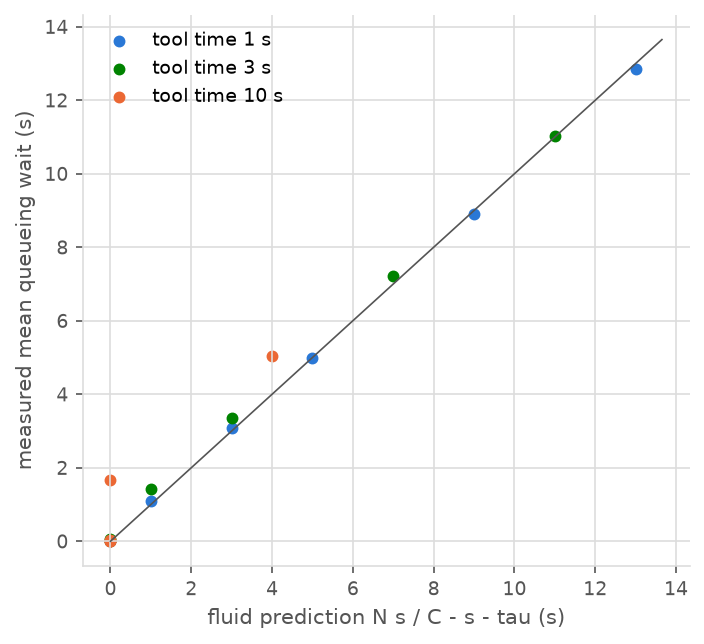
\includegraphics[width=0.75\columnwidth]{figA6_fluid.png}
  \caption{Measured mean queueing wait against $Ns/C-s-\tau$ for $N\in\{16,\dots,128\}$ and three tool times.}
  \label{fig:fluid}
\end{figure}

\section{Evaluation}\label{sec:eval}
Defaults: $C{=}16$, $K{=}64$, 10 seeds, median and interquartile range. Task capacity is 1.33 tasks/s. Everything is simulated; \cref{sec:limits} lists what that means.

\subsection{Overload}\label{sec:overload}
\begin{figure*}[t]\centering
  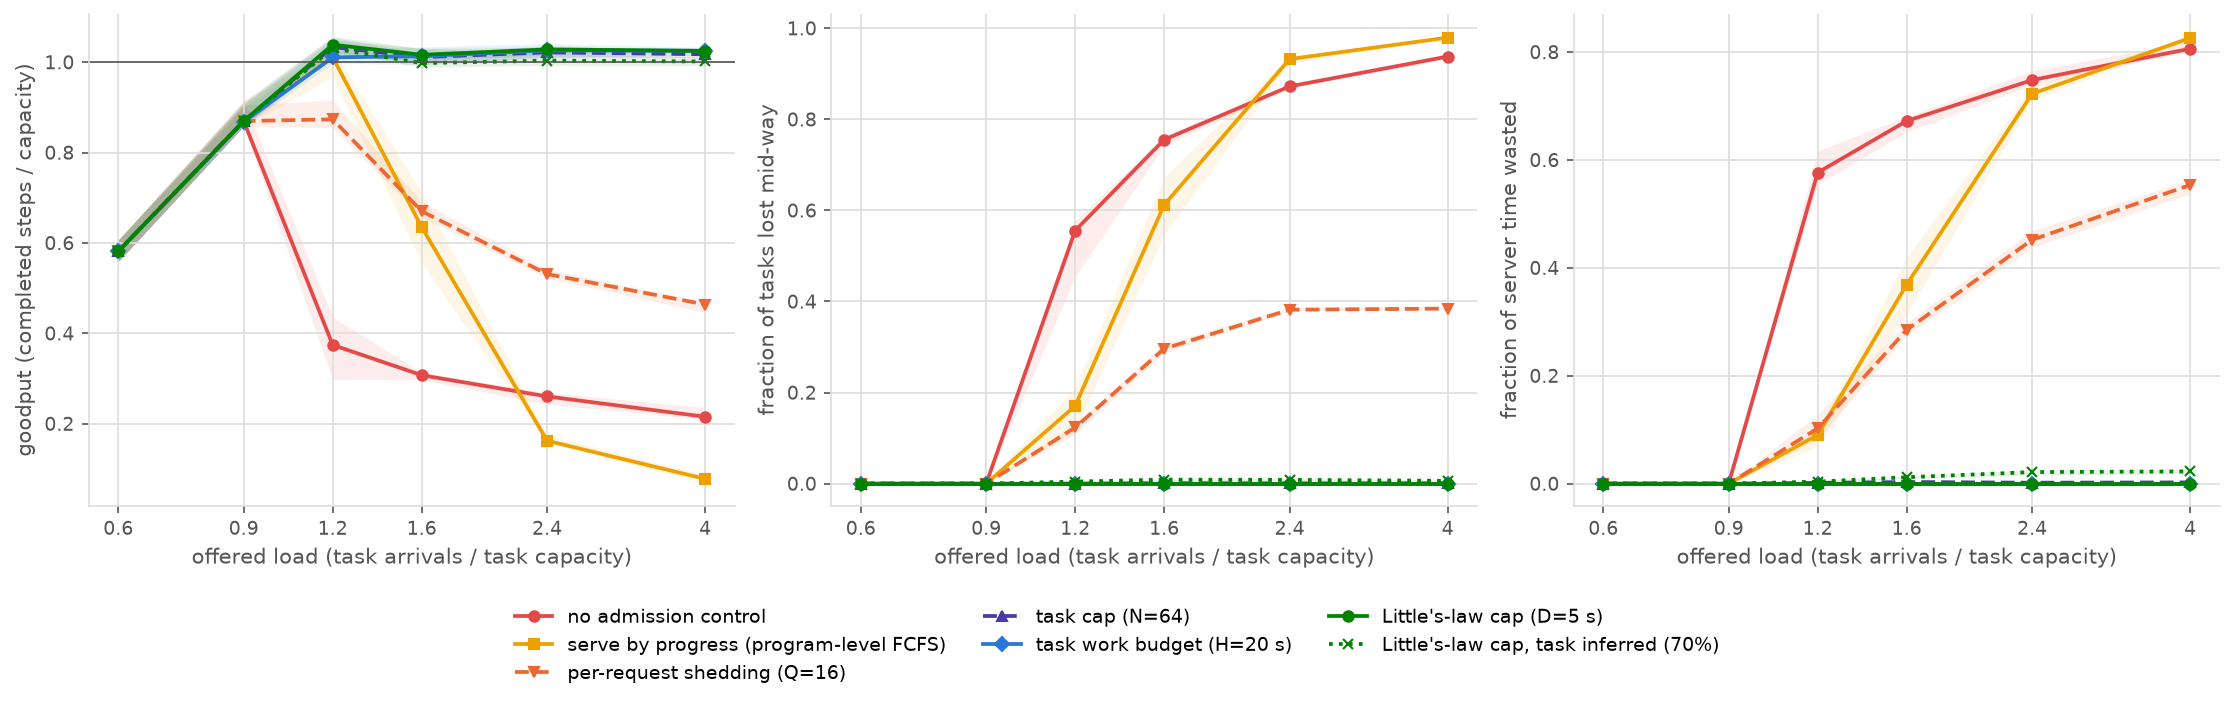
\includegraphics[width=\textwidth]{figA1_overload.png}
  \caption{Goodput, tasks lost mid-way and wasted server time against offered load.}
  \label{fig:overload}
\end{figure*}
\Cref{fig:overload} shows the failure. Without admission control, goodput falls from 0.87 at 0.9$\times$ to 0.37 at 1.2$\times$ and 0.26 at 2.4$\times$; 87\% of tasks are lost mid-way and 75\% of server time is wasted. Serving by progress helps at mild overload (1.01 at 1.2$\times$) but collapses at 2.4$\times$ (0.16): the oldest tasks are served first, but the queue still outgrows the timeout. Per-request shedding with $Q{=}16$ keeps 0.53 at 2.4$\times$ but still loses 38\% of tasks mid-way, because it rejects steps of tasks it already accepted. A task cap ($N{=}64$), the work budget ($H{=}20$\,s) and the Little's-law cap all hold 1.00--1.03 of capacity from 1.2$\times$ to 4$\times$ with no task lost mid-way and under 1\% of server time wasted. The price is rejecting new tasks: at 4$\times$ only 25\% of arriving tasks complete, the rest being refused at the door instead of after wasted work. Completed tasks have a P99 latency of 214\,s (vs.\ 312\,s with no control).

\subsection{Tuning}
\begin{figure}[t]\centering
  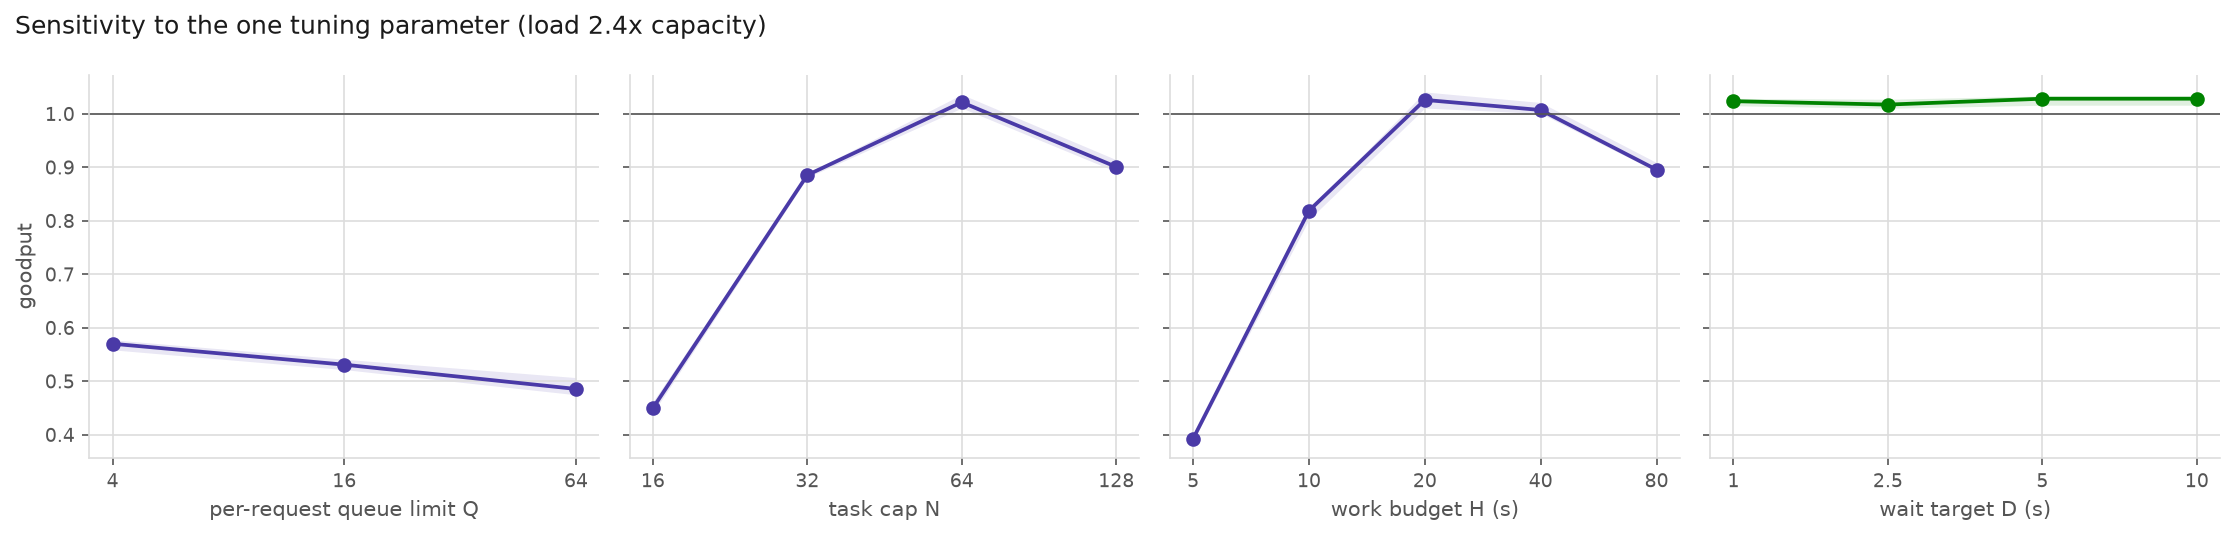
\includegraphics[width=\columnwidth]{figA2_sensitivity.png}
  \caption{Goodput at 2.4$\times$ overload against each rule's tuning parameter.}
  \label{fig:sens}
\end{figure}
\Cref{fig:sens} shows sensitivity at 2.4$\times$ overload. Per-request shedding never exceeds 0.57. A task cap is good only for $N$ near 64 (0.45 at 16, 0.89 at 32, 0.90 at 128). The work budget is good for $H\in[20,40]$\,s. The Little's-law cap holds 1.02--1.03 for every $D$ from 1 to 10\,s.
\Cref{fig:regimes} sweeps 81 regimes at 2.4$\times$ overload (mean task length 3/6/12, tool time 1/3/10\,s, timeout 15/30/60\,s, KV capacity 16/64/256 tasks). We choose each fixed parameter on seeds 0--4 and evaluate on seeds 5--9, scoring goodput against the best policy in each regime. The best $N$ for the task cap is 64 in 29 regimes, 32 in 23, 128 in 16 and 16 in 13; no single value is safe: one fixed $N$ has a 10th percentile of 0.62 of the best. The Little's-law cap with $D{=}5$ and no tuning has median 0.99 and is within 0.9 of the best in 85\% of regimes, against 91\% for a cap tuned per regime and 65\% for one fixed cap. Per-request shedding reaches 0.68 of the best at the median and no admission control 0.15.
\begin{figure}[t]\centering
  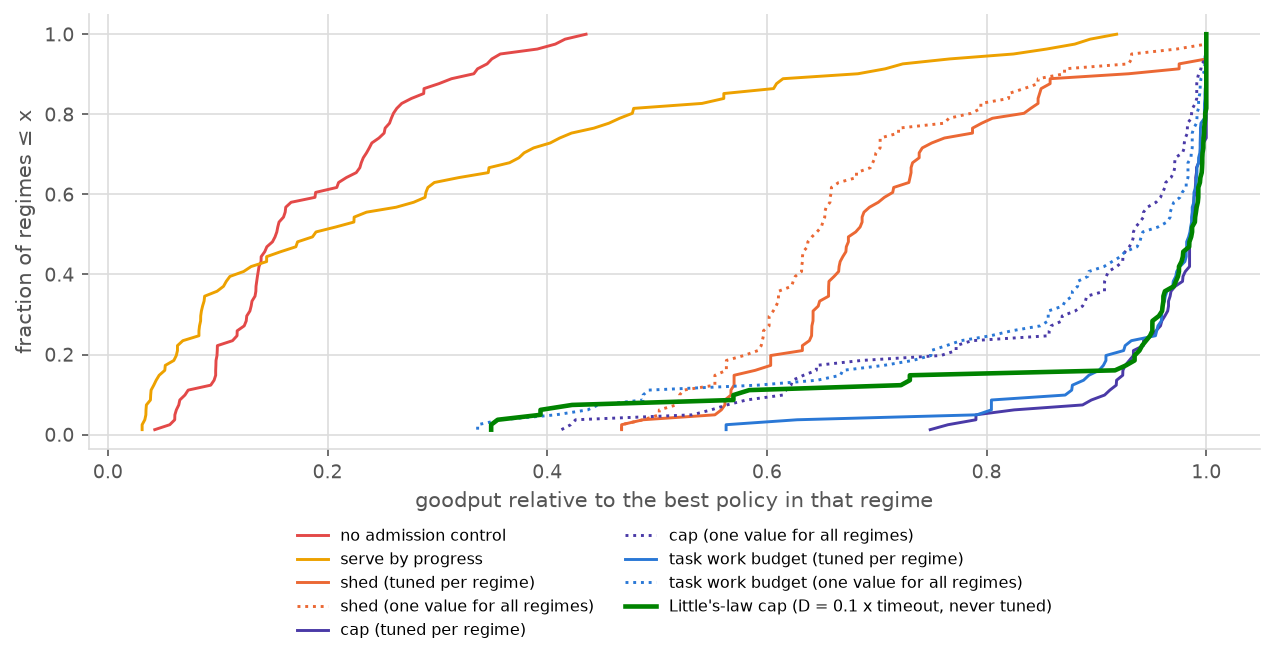
\includegraphics[width=\columnwidth]{figA4_regimes.png}
  \caption{Goodput relative to the best policy per regime across 81 regimes.}
  \label{fig:regimes}
\end{figure}
The Little's-law cap's weak regimes are KV-bound: its 10th percentile is 0.58 and its worst case 0.35, all 12 such regimes have a KV capacity of 16 tasks, where a cap that admits more tasks than fit in KV and accepts rebuild costs does better. We tried admitting up to 2$\times$ or 4$\times$ the KV capacity and it was worse overall.

\subsection{What task information is worth}
\begin{figure}[t]\centering
  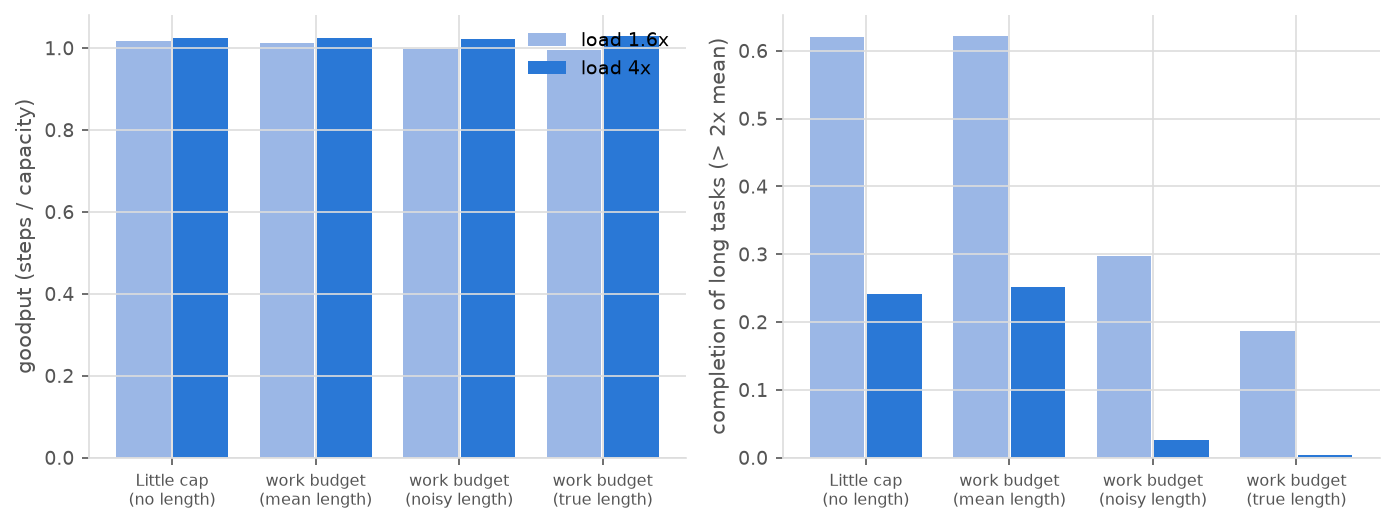
\includegraphics[width=\columnwidth]{figA5_information.png}
  \caption{Work goodput and long-task completion for different knowledge of task length.}
  \label{fig:info}
\end{figure}
Knowing task lengths seems useful: with exact lengths the work budget completes 2.28$\times$ the task capacity in tasks at 4$\times$ load (noisy lengths, $\sigma{=}0.5$: 2.12$\times$), because it admits short tasks. But work goodput is the same (1.02--1.03), and long tasks (more than twice the mean) are starved: only 0\% (exact) and 3\% (noisy) complete, against 24\% for the length-free cap (\cref{fig:info}). Length information therefore buys a count of completed tasks, not capacity, at the cost of fairness. Identity matters less than expected: recognising 70\% of steps (the rest treated as new tasks, so sometimes refused mid-task) loses 2\% of goodput at 4$\times$; recognising 50\% loses 12\%.

\subsection{Surges and retries}
After a 60\,s surge of 3$\times$ and 5$\times$ base load, only the unprotected server stays degraded: 55\% and 60\% of later tasks complete, against 100\% for the default setting of each protected policy (serving by progress: 94\% after a 5$\times$ surge; a badly tuned queue limit $Q{=}64$ or cap $N{=}16$: 75\% and 55\%). In our model, per-request shedding with a tight queue limit also recovers, so the surge test separates only unprotected servers from protected ones. A retry sweep (0, 1, 3 or 8 retries, backoff 0.5, 2 or 8\,s) is in the artifact summary.

\section{Related Work}
Overload control for services is a mature area: SEDA bounds queues per stage~\citep{welsh2001seda}, DAGOR sheds load by priority using queueing time~\citep{zhou2018dagor}, and Breakwater uses server-issued credits driven by queueing delay~\citep{cho2020breakwater}. Metastable failures from retry amplification are documented in production~\citep{bronson2021metastable,huang2022metastable}. Our rule is in this family, a delay-targeted concurrency limit; what is specific here is the unit (a multi-step task whose abandonment wastes accumulated work), the closed-population formula that accounts for tool time, and the KV-memory bound. Agent-serving systems reduce latency by pinning or prefetching KV state and prioritising program progress~\citep{continuum2025,tokencake2025,saga2026,cachewise2026}; they target throughput and completion time, not admission under overload, and \emph{prog} in our evaluation is a minimal version of their scheduling idea.

\section{Limitations}\label{sec:limits}
All results come from one simulated server; there is no real GPU, batching or decode model, and no real agent trace (we found no public one with task boundaries, so arrivals are Poisson and tool times exponential). Parameters are plausible, not measured. We do not model priorities, deadlines or multiple replicas; with many routers the admission state would itself be shared stale state, the herding setting of the companion paper. The Little's-law cap needs task identity to count tasks and to measure $\tau$, and it is conservative when KV memory binds. The recovery experiment does not separate good protected policies.

\section{Conclusion}
Under overload, agents make admission a per-task decision: a refused task costs nothing, an abandoned one wastes everything. Counting admitted tasks against a Little's-law cap holds the queueing wait at a chosen target, keeps goodput near capacity, and needs neither length prediction nor careful tuning, but it relies on knowing which request belongs to which task and on KV memory not being the binding constraint.

\bibliographystyle{plainnat}
\bibliography{refs}
\end{document}
